\documentclass[UTF8]{ctexart}
\usepackage[a4paper,left=3cm,right=3cm,top=2cm]{geometry}
\usepackage{amsmath}
\usepackage{enumitem}
\usepackage{float}
\usepackage{threeparttable}
\usepackage{caption}
\usepackage{multirow}
\usepackage{graphicx}
\usepackage{listings}
\usepackage{color}
\definecolor{dkgreen}{rgb}{0,0.6,0}
\definecolor{gray}{rgb}{0.5,0.5,0.5}
\definecolor{mauve}{rgb}{0.58,0,0.82}
\lstset{frame=tb,
  language=Python,
  aboveskip=3mm,
  belowskip=3mm,
  showstringspaces=false,
  columns=flexible,
  basicstyle={\small\ttfamily},
  numbers=left,%设置行号位置none不显示行号
  %numberstyle=\tiny\courier, %设置行号大小
  numberstyle=\tiny\color{gray},
  keywordstyle=\color{blue},
  commentstyle=\color{dkgreen},
  stringstyle=\color{mauve},
  breaklines=true,
  breakatwhitespace=true,
  tabsize=4,
  extendedchars=false %解决代码跨页时,章节标题,页眉等汉字不显示的问题
}

\setlength\lineskiplimit{5.25bp}
\setlength\lineskip{5.25bp}

\title{利用Python进行天体运行的模拟}
\author{崔士强 PB22151743}
\date{\today}

\bibliographystyle{plain}

\begin{document}

\maketitle
\section{原理}
本程序通过设置步长再逐步计算的方式进行模拟. 设步长为$dt$,两个天体的位置坐标分别为$\mathbf{p}_i$, $\mathbf{p}_j$
每一步需要进行的计算为:
\[\mathbf{F}_{ij,t}=\frac{Gm_im_j}{d^2}\mathbf{e}_{ij}\]
\[\mathbf{a}_{ij,t}=\frac{\mathbf{F}_{ij,t}}{m_i}\]
\[\mathbf{v}_{i,t+1}=\mathbf{v}_{i,t}+\mathbf{a}_{i,t}dt\]
可以计算两个天体经过一小段时间的位置变化(近似值).

程序还涉及添加环绕天体. 结合向心力公式
\[F=\frac{mv^2}{R}\]
可以得到
\[v=\sqrt{\frac{GM}{R}}\]
其中$M$为中心天体质量. 添加环绕天体时同时赋予该速度.
\section{设计方案}
定义一个类CelestialBody来表示天体. 属性包括名称name,质量mass,位置position,速度velocity,
两个方法update\_velocity和update\_position分别计算速度和位置的变化。

对于每一个输入的质量及长度,提供几个可选单位,程序中用一个字典存储这些单位,输入后由函数
convert\_mass\_to\_kg以及convert\_distance\_to\_m换算成国际单位制。

如果添加环绕天体,程序会将其放置在中心天体x负方向,距离(即环绕半径)由用户输入。
程序根据中心天体质量以及环绕半径计算速度。

如果发射一个天体,用户需要输入发射起点,方向以及速度。程序会计算三个方向上的分速度。

添加天体完成后可以选择进行模拟。需要输入步长以及步数。程序逐步计算,每一步的结果储存在二维列表positions中。
每一步计算完成后检查是否出现相撞。判定标准为两个天体小于用户输入的阈值即为相撞,根据动量守恒计算相撞后运动情况,
这里假设撞后两个天体合二为一。

模拟完成后可以绘图表示结果。程序根据列表positions的信息绘制散点图,图中的点即为每一步各个天体的位置
\section{创新性描述}
\begin{enumerate}
  \item 程序为质量和长度提供了多个单位,方便输入
  \item 通过局部近似成匀速直线运动进行模拟,避免过于复杂的计算
\end{enumerate}
\section{运行示例}
两个质量均为1倍太阳质量的天体a,b. a静止于原点,b于$(0.5AU, 0.5AU, 0.5AU)$的位置,以$20\mathrm{km/s^2}$
的速度向z轴负方向射出,模拟步长为$5000\mathrm{s}$,模拟1000步,结果如下图所示:
\begin{figure}[h]
  \centering
  \includegraphics[scale=0.6]{sim.png}
  \caption{示例结果1}
\end{figure}

如果将步数增加至4000步,结果如下图所示:
\begin{figure}[h]
  \centering
  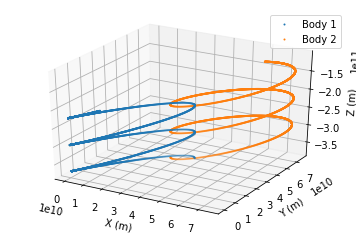
\includegraphics[scale=0.6]{sim2.png}
  \caption{示例结果2}
\end{figure}
\section{学习心得}
本课程是我接触的第二门计算机类课程,使我了解了又一种计算机语言Python。相比于C语言,Python丰富的科学计算
库,更高的开发效率使得其在多数场景下更适合科学计算。通过本课程,我获取了辅助日常学习以及今后科研工作
的一项重要技能,也接触到了面向对象编程的思想。

\begin{thebibliography}{5}
  \bibitem{ref1}罗奇鸣. Python科学计算基础.
  \bibitem{ref2}Ian Morison. Introduction to Astronomy and Cosmology. West Sussex: John Wiley \& Sons Ltd, 2008.
\end{thebibliography}

\bibliography{math}

\end{document}
\iffalse
\begin{figure}[h]
    \centering
    \includegraphics[scale=0.5]{name.png}
    \caption{name}
\end{figure}
\fi
